\documentclass{beamer}
\usepackage{algpseudocode}
\title{Algorithmic Methods for Mathematical Models\\
 Course Project}
\author{Marco Bartoli, Ilan Vezmarovic}
\institute{UPC Universitat Politècnica de Catalunya}
\date{\today}

\makeatletter
\algrenewcommand\ALG@beginalgorithmic{\footnotesize}
\makeatother

\begin{document}

\frame{\titlepage}

\begin{frame}
\frametitle{Formal Problem Definition}
\begin{itemize}
    \item $n$: number of products
    \item $x$: height of the suitcase in millimeters
    \item $y$: width of the suitcase in millimeters
    \item $c$: limit to the total weight of the suitcase in grams
    \item $p_i$: price of the $i$-th product in euros
    \item $w_i$: weight of the $i$-th product in grams
    \item $s_i$: side length of the $i$-th product's (square) box in millimeters
\end{itemize}
\end{frame}


\begin{frame}
\frametitle{Decision Variables}
\begin{itemize}
    \item $\text{Chosen}_i$: binary variable that is 1 if object $i$ is chosen, and 0 otherwise.
    \item $\text{PointsX}_i$: the x-coordinate of the bottom-left corner of object $i$.
    \item $\text{PointsY}_i$: the y-coordinate of the bottom-left corner of object $i$.
    \item $\text{Overlap}_{i,j,d}$: binary variable indicating if objects $i$ and $j$ do not overlap in direction $d$, where $d \in \{1, 2, 3, 4\}$.
\end{itemize}
\end{frame}

\begin{frame}
\frametitle{Objective Function}
Maximize the total price of the chosen objects:

\[
\text{maximize} \sum_{i=1}^n p_i \cdot \text{Chosen}_i
\]
\end{frame}


\begin{frame}
\frametitle{Max Weight Constraint}
Ensure the total weight of the chosen objects does not exceed the suitcase's capacity:

\[
\sum_{i=1}^n w_i \cdot \text{Chosen}_i \leq c
\]
\end{frame}

\begin{frame}
\frametitle{Coordinate Bounds Constraints}
Ensure each object lies entirely within the suitcase's boundaries:

\[
\forall i \in \{1, \ldots, n\}, \quad \text{PointsX}_i \geq 1
\]

\[
\forall i \in \{1, \ldots, n\}, \quad \text{PointsY}_i \geq 1
\]

\[
\forall i \in \{1, \ldots, n\}, \quad \text{PointsX}_i + s_i - 1 \leq x
\]

\[
\forall i \in \{1, \ldots, n\}, \quad \text{PointsY}_i + s_i - 1 \leq y
\]
\end{frame}


\begin{frame}
\frametitle{Non-Overlapping Constraints}
Left/Right/Up/Down non-overlapping:


\[
\forall i, j \in \{1, \ldots, n\}, i \neq j, \quad \text{PointsX}_i - \text{PointsX}_j + s_i \leq
\]
\[
-M \cdot (\text{Chosen}_i + \text{Chosen}_j + \text{Overlap}_{i,j,1} - 3)
\]

\[
\forall i, j \in \{1, \ldots, n\}, i \neq j, \quad \text{PointsX}_i - \text{PointsX}_j + s_i \leq
\]
\[
-M \cdot (\text{Chosen}_i + \text{Chosen}_j + \text{Overlap}_{i,j,2} - 3)
\]

\[
\forall i, j \in \{1, \ldots, n\}, i \neq j, \quad \text{PointsX}_i - \text{PointsX}_j + s_i \leq
\]
\[
-M \cdot (\text{Chosen}_i + \text{Chosen}_j + \text{Overlap}_{i,j,3} - 3)
\]

\[
\forall i, j \in \{1, \ldots, n\}, i \neq j, \quad \text{PointsX}_i - \text{PointsX}_j + s_i \leq
\]
\[
-M \cdot (\text{Chosen}_i + \text{Chosen}_j + \text{Overlap}_{i,j,4} - 3)
\]
\end{frame}

\begin{frame}{Non-Overlapping Constraints}
At least one of the non-overlapping conditions is satisfied:

\[
\forall i, j \in \{1, \ldots, n\}, i \neq j, \quad \sum_{d=1}^4 \text{Overlap}_{i,j,d} \geq 1
\]
    
\end{frame}


\begin{frame}[fragile] 
\frametitle{Greedy heuristic}
\begin{algorithm}
\begin{algorithmic}
    \State \textbf{Input:} A problem instance with $n$ products, suitcase dimensions $(x, y)$, and weight capacity $c$.
    \State \textbf{Output:} A feasible solution with selected products that maximize the total price.    

    \State Initialize solution as empty
    \State Sort products by $(price / side / weight)$ in descending order

    \For{each product in sorted products}
        \If{product can fit in the suitcase and does not exceed weight limit}
            \State Add product to solution
            \State Update suitcase dimensions and weight capacity
        \EndIf
    \EndFor

    \State \Return solution
\end{algorithmic}
\end{algorithm}

\end{frame}


\begin{frame}[fragile] 
\frametitle{Local search}
\begin{algorithm}
\begin{algorithmic}
   \State \textbf{Input:} An initial solution, mode and strategy.
    \State \textbf{Output:} An improved solution

    \State bestSolution = initialSolution
    \State improved = true
        
    \While{improved}
        \State improved = false

        \For{each product in bestSolution}
            \If{strategy == EXCHANGE}
                \State newSolution = exchangeProduct(bestSolution, product)
            \ElsIf{strategy == REASSIGNMENT}
                \State newSolution = reassignProduct(bestSolution, product)
            \EndIf

            \If{newSolution is better than bestSolution}
                \State bestSolution = newSolution
                \State improved = true
                
                \If{mode == FIRST\_IMPROVEMENT}
                    \State \Return bestSolution
                \EndIf
            \EndIf
        \EndFor
    \EndWhile

    \State \Return bestSolution
\end{algorithmic}
\end{algorithm}

\end{frame}


\begin{frame}
\frametitle{Local Search Time chart}
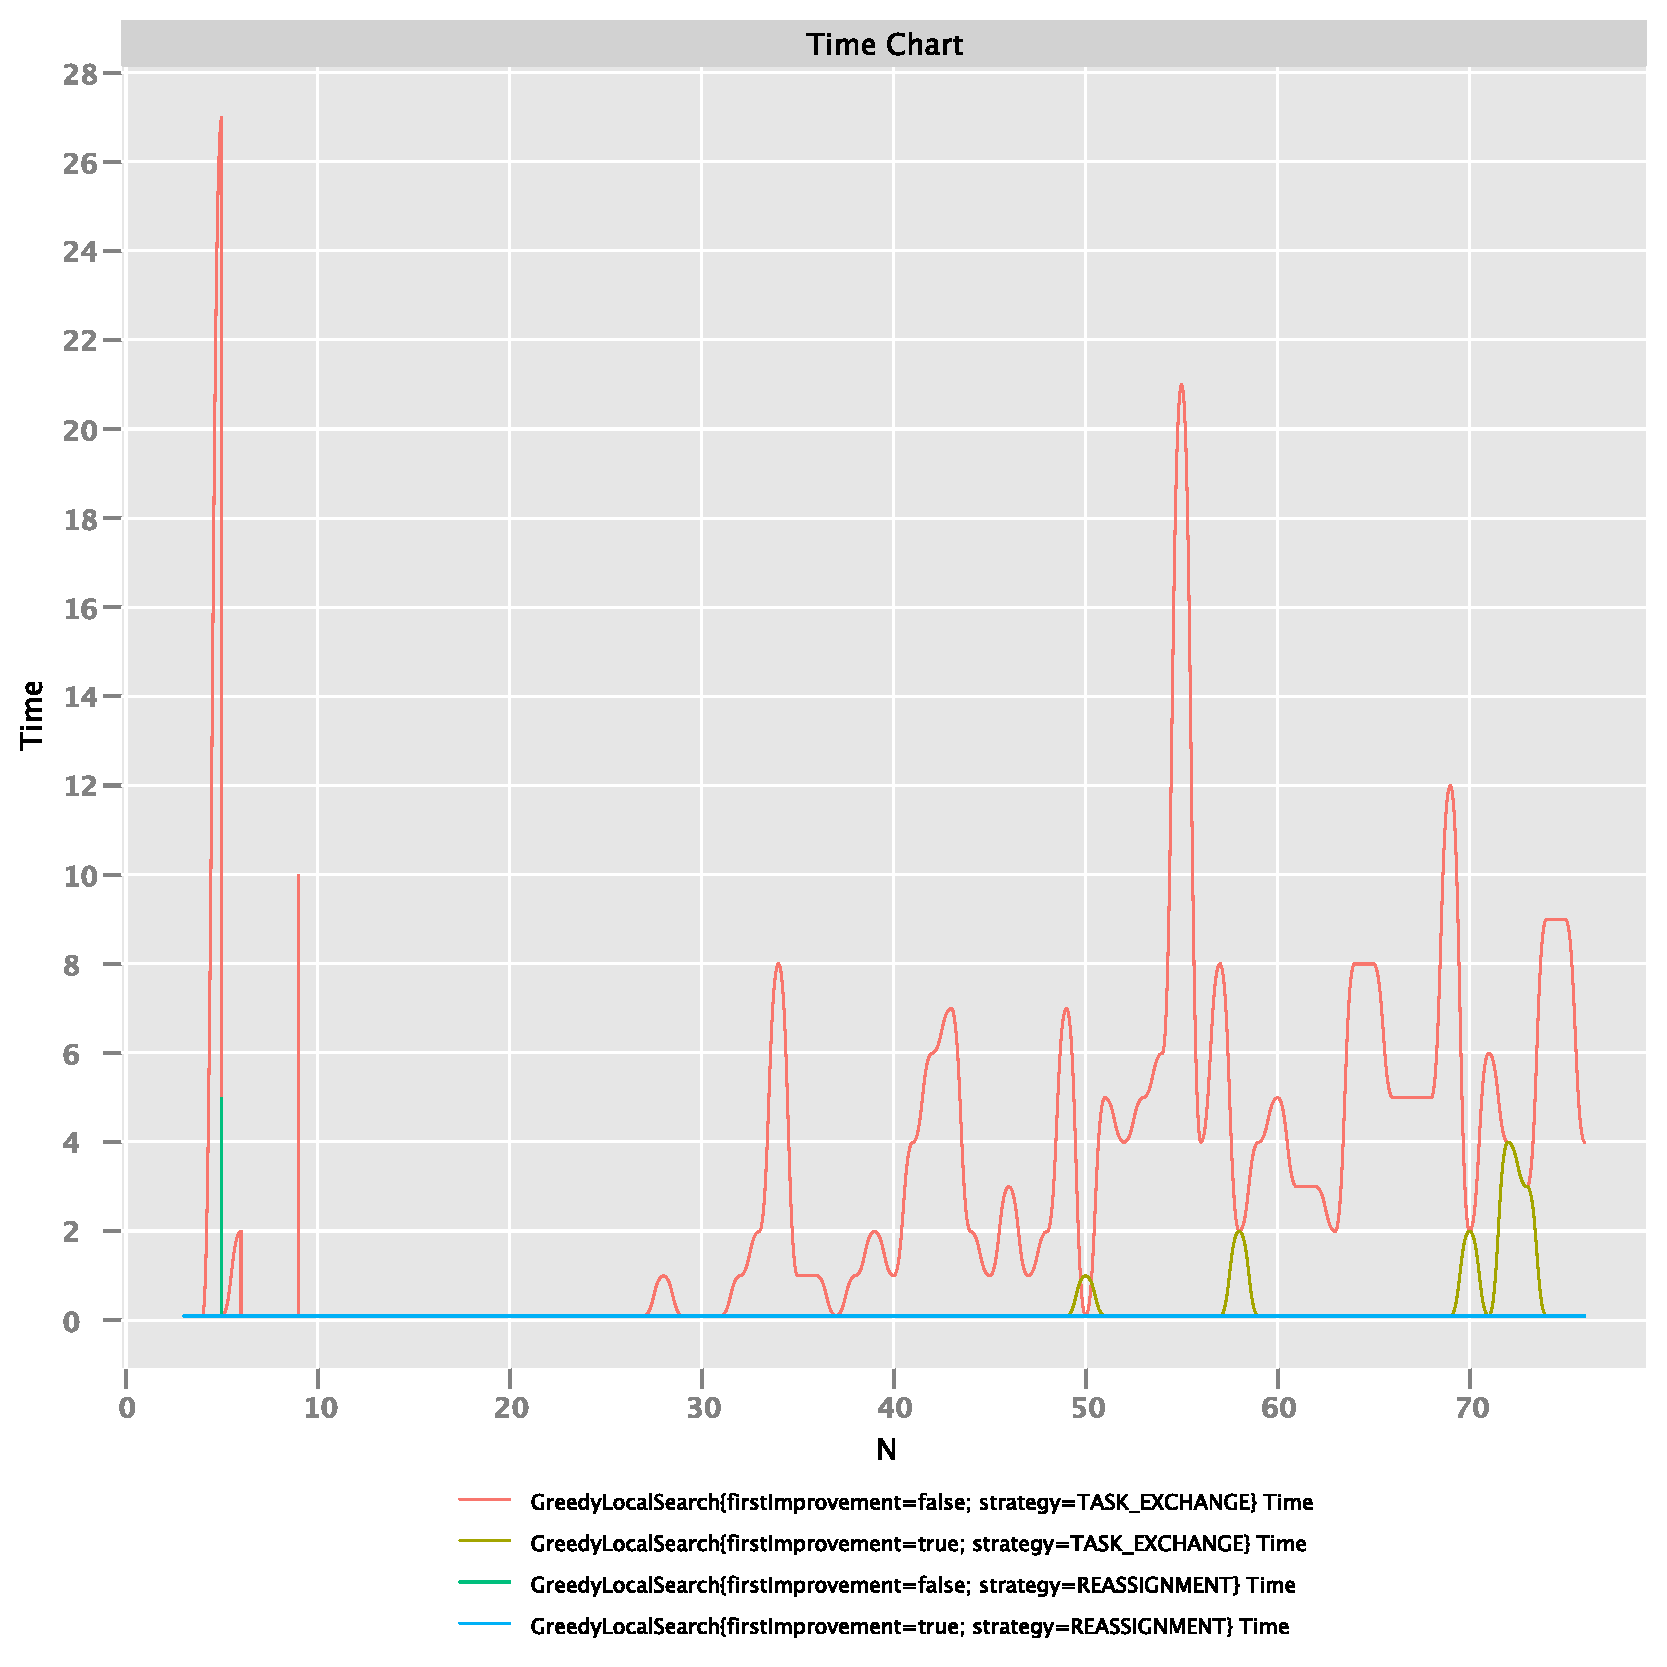
\includegraphics[width=0.8\textwidth]{./documentation/assets/new.localSearchParams.timeChart.pdf}
\end{frame}

\begin{frame}
\frametitle{Local Search Objective chart}
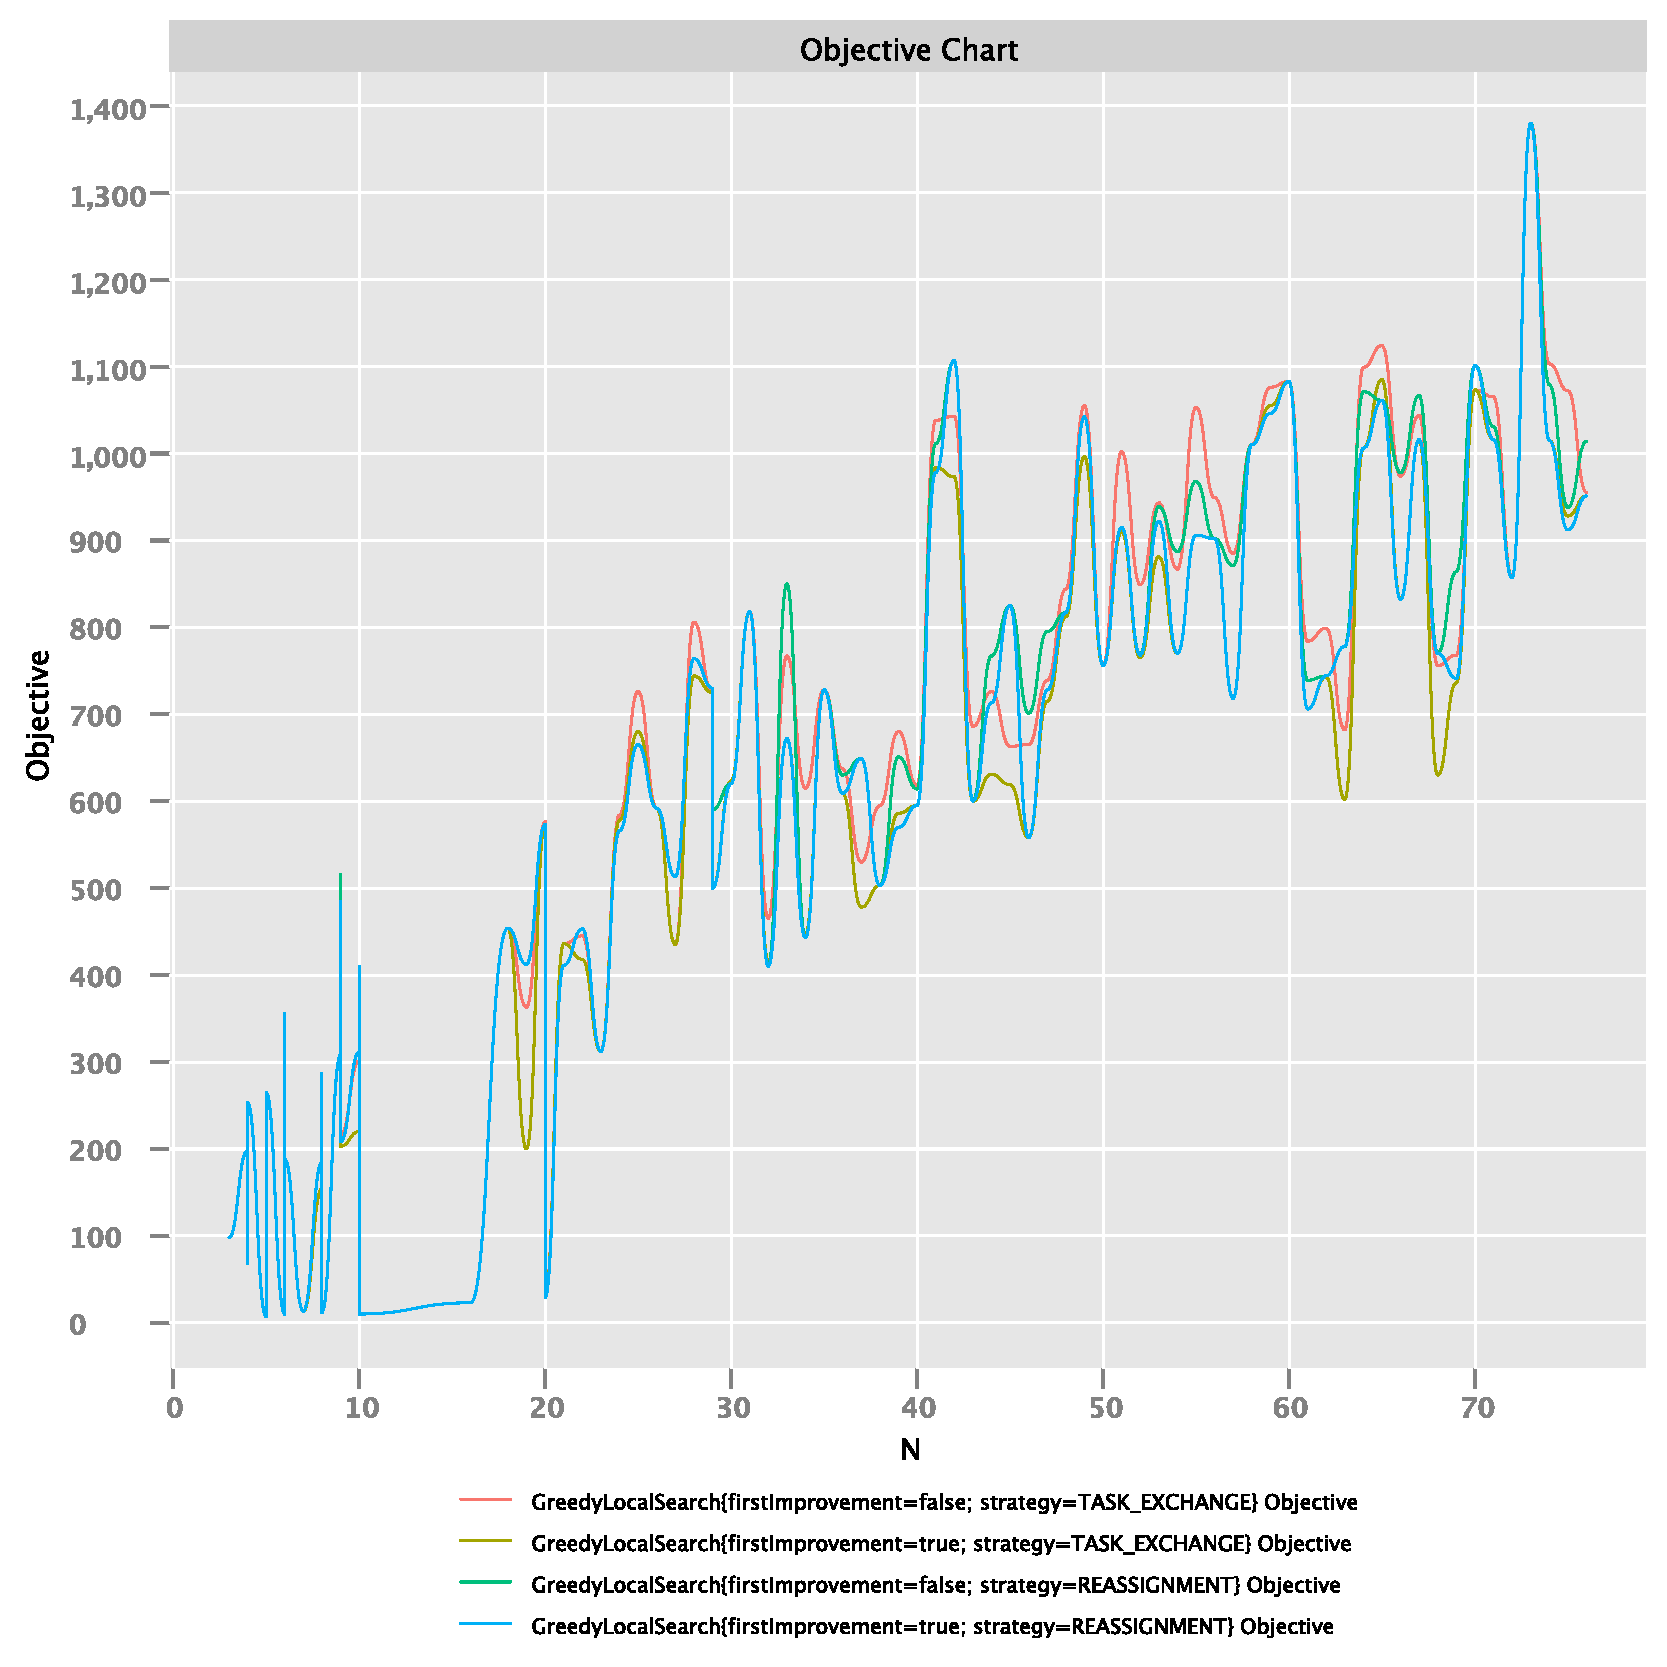
\includegraphics[width=0.8\textwidth]{./documentation/assets/new.localSearchParams.objectiveChart.pdf}
\end{frame}

\begin{frame}[fragile] 
\frametitle{GRASP}
\begin{algorithm}
\begin{algorithmic}
    \State \textbf{Input:} A problem instance, maxIterations, alpha (for RCL threshold)
    \State \textbf{Output:} The best solution found

    \State bestSolution = null

    \For{iteration = 1 to maxIterations}
        \State greedySolution = constructGreedyRandomizedSolution(problem, alpha)
        \State localOptimalSolution = LOCAL\_SEARCH(greedySolution, FIRST\_IMPROVEMENT)

        \If{bestSolution is null or localOptimalSolution is better than bestSolution}
            \State bestSolution = localOptimalSolution
        \EndIf
    \EndFor

    \State \Return bestSolution
\end{algorithmic}
\end{algorithm}
\end{frame}

\begin{frame}[fragile] 
\frametitle{GRASP (2)}
\begin{algorithm}
\begin{algorithmic}
    \State \textbf{Input:} A problem instance, alpha (for RCL threshold)
    \State \textbf{Output:} A feasible solution

    \State Initialize solution as empty
    \State Sort products by $(price / side / weight)$ in descending order

    \While{there are remaining products}
        \State $qMax$ = maximum $Q$ value in remaining products
        \State $qMin$ = minimum $Q$ value in remaining products
        \State threshold = $qMax - alpha \times (qMax - qMin)$

        \State RCL = \{products with $Q$ value $>=$ threshold\}
        \State selectedProduct = randomly select a product from RCL

        \If{selectedProduct fits in the suitcase and does not exceed weight limit}
            \State Add selectedProduct to solution
            \State Update suitcase dimensions and weight capacity
        \EndIf
    \EndWhile

    \State \Return solution
\end{algorithmic}
\end{algorithm}

\end{frame}

\begin{frame}
\frametitle{GRASP Time chart}
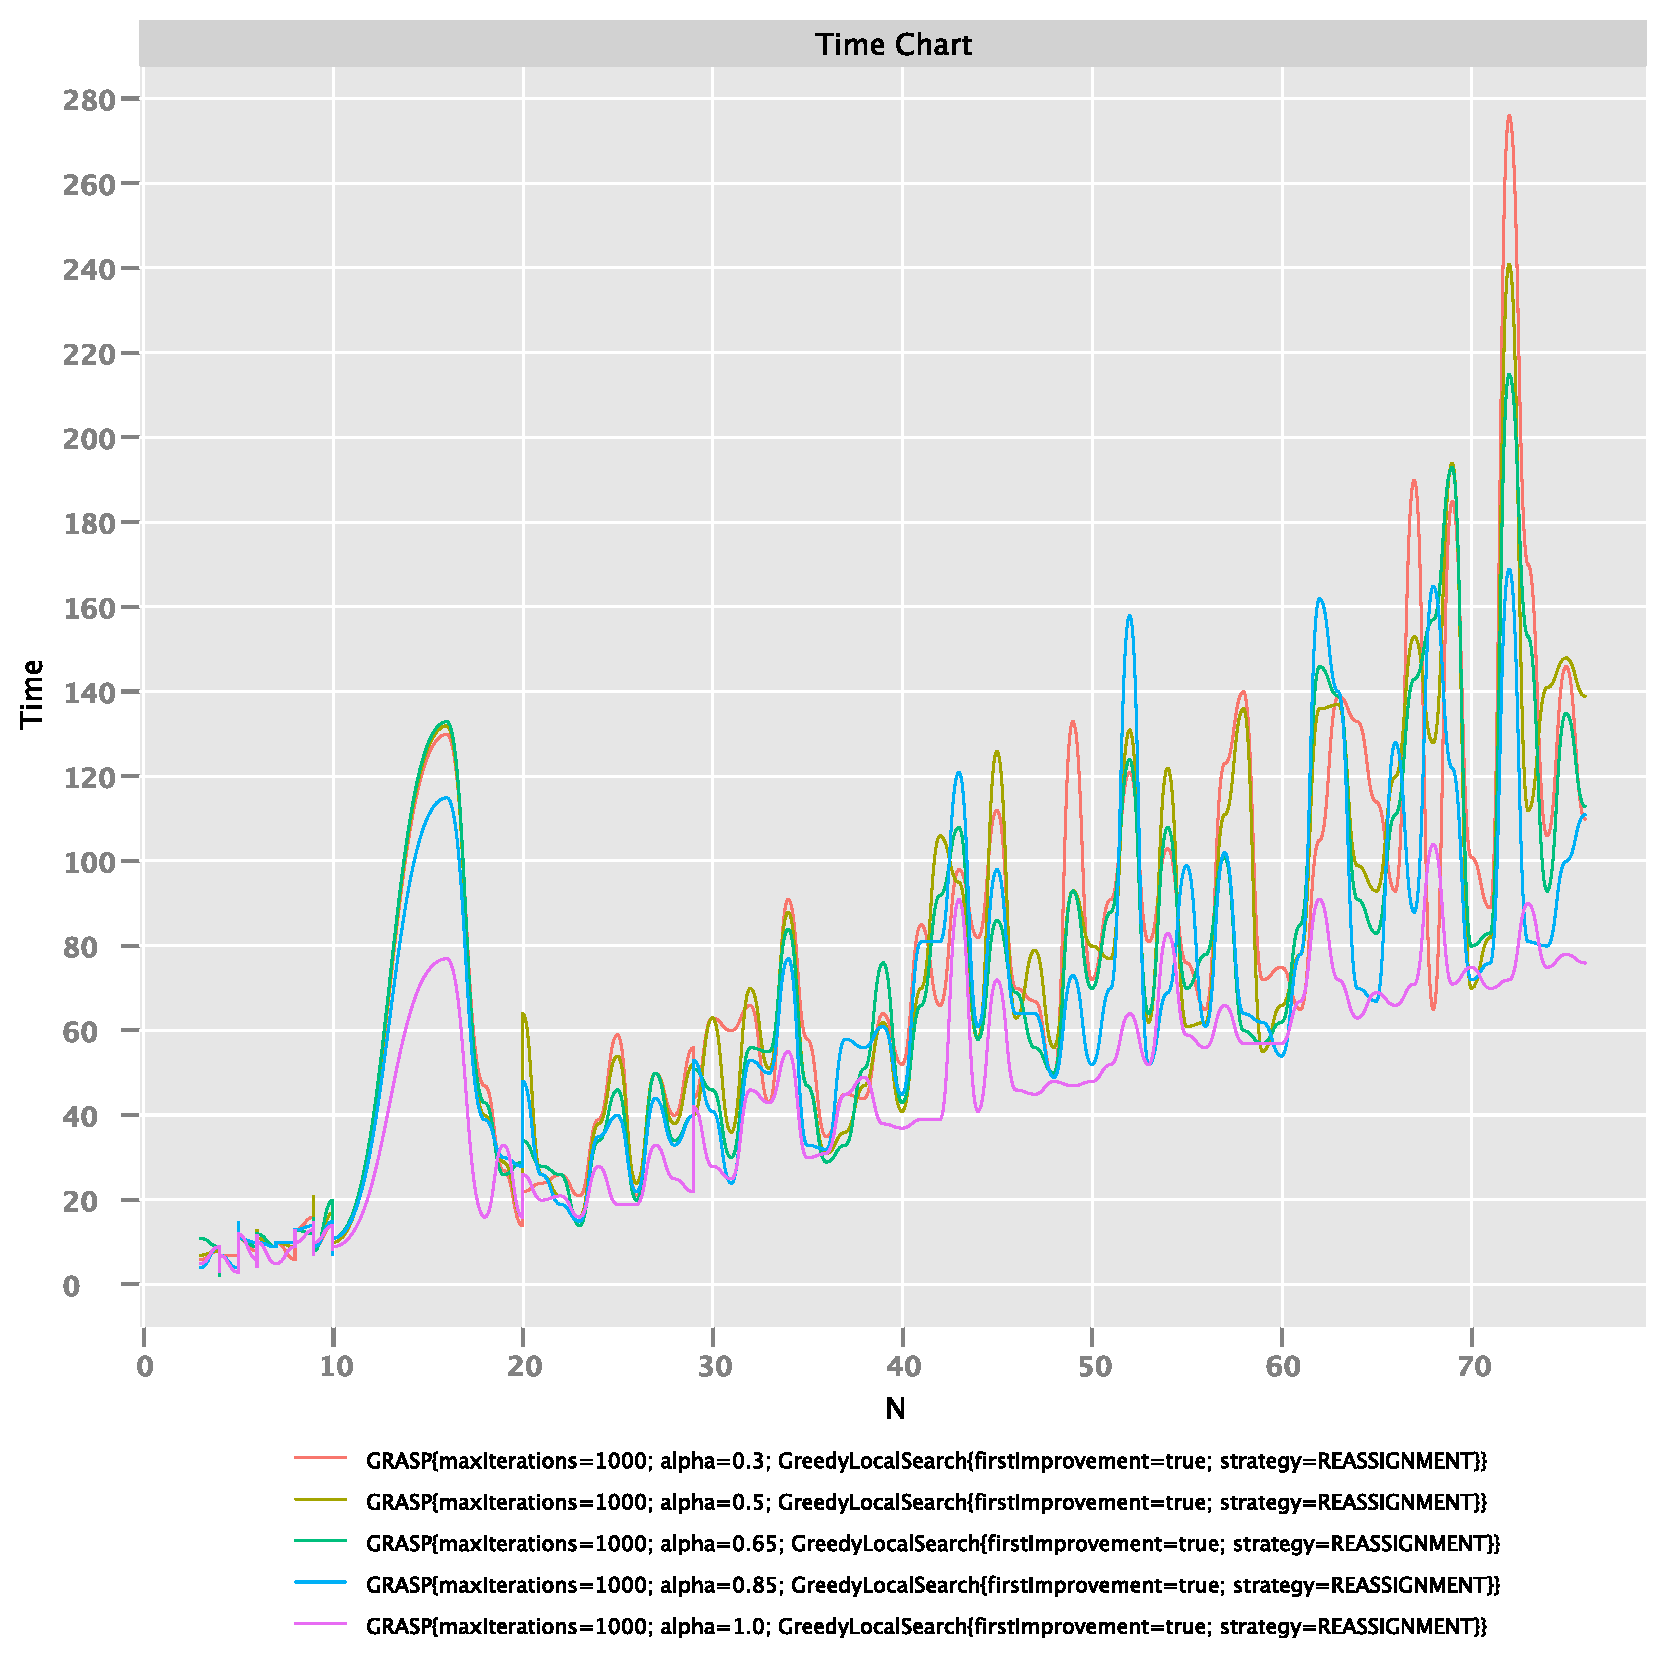
\includegraphics[width=0.8\textwidth]{./documentation/assets/new.GRASPParams.timeChart.pdf}
\end{frame}

\begin{frame}
\frametitle{GRASP Objective chart}
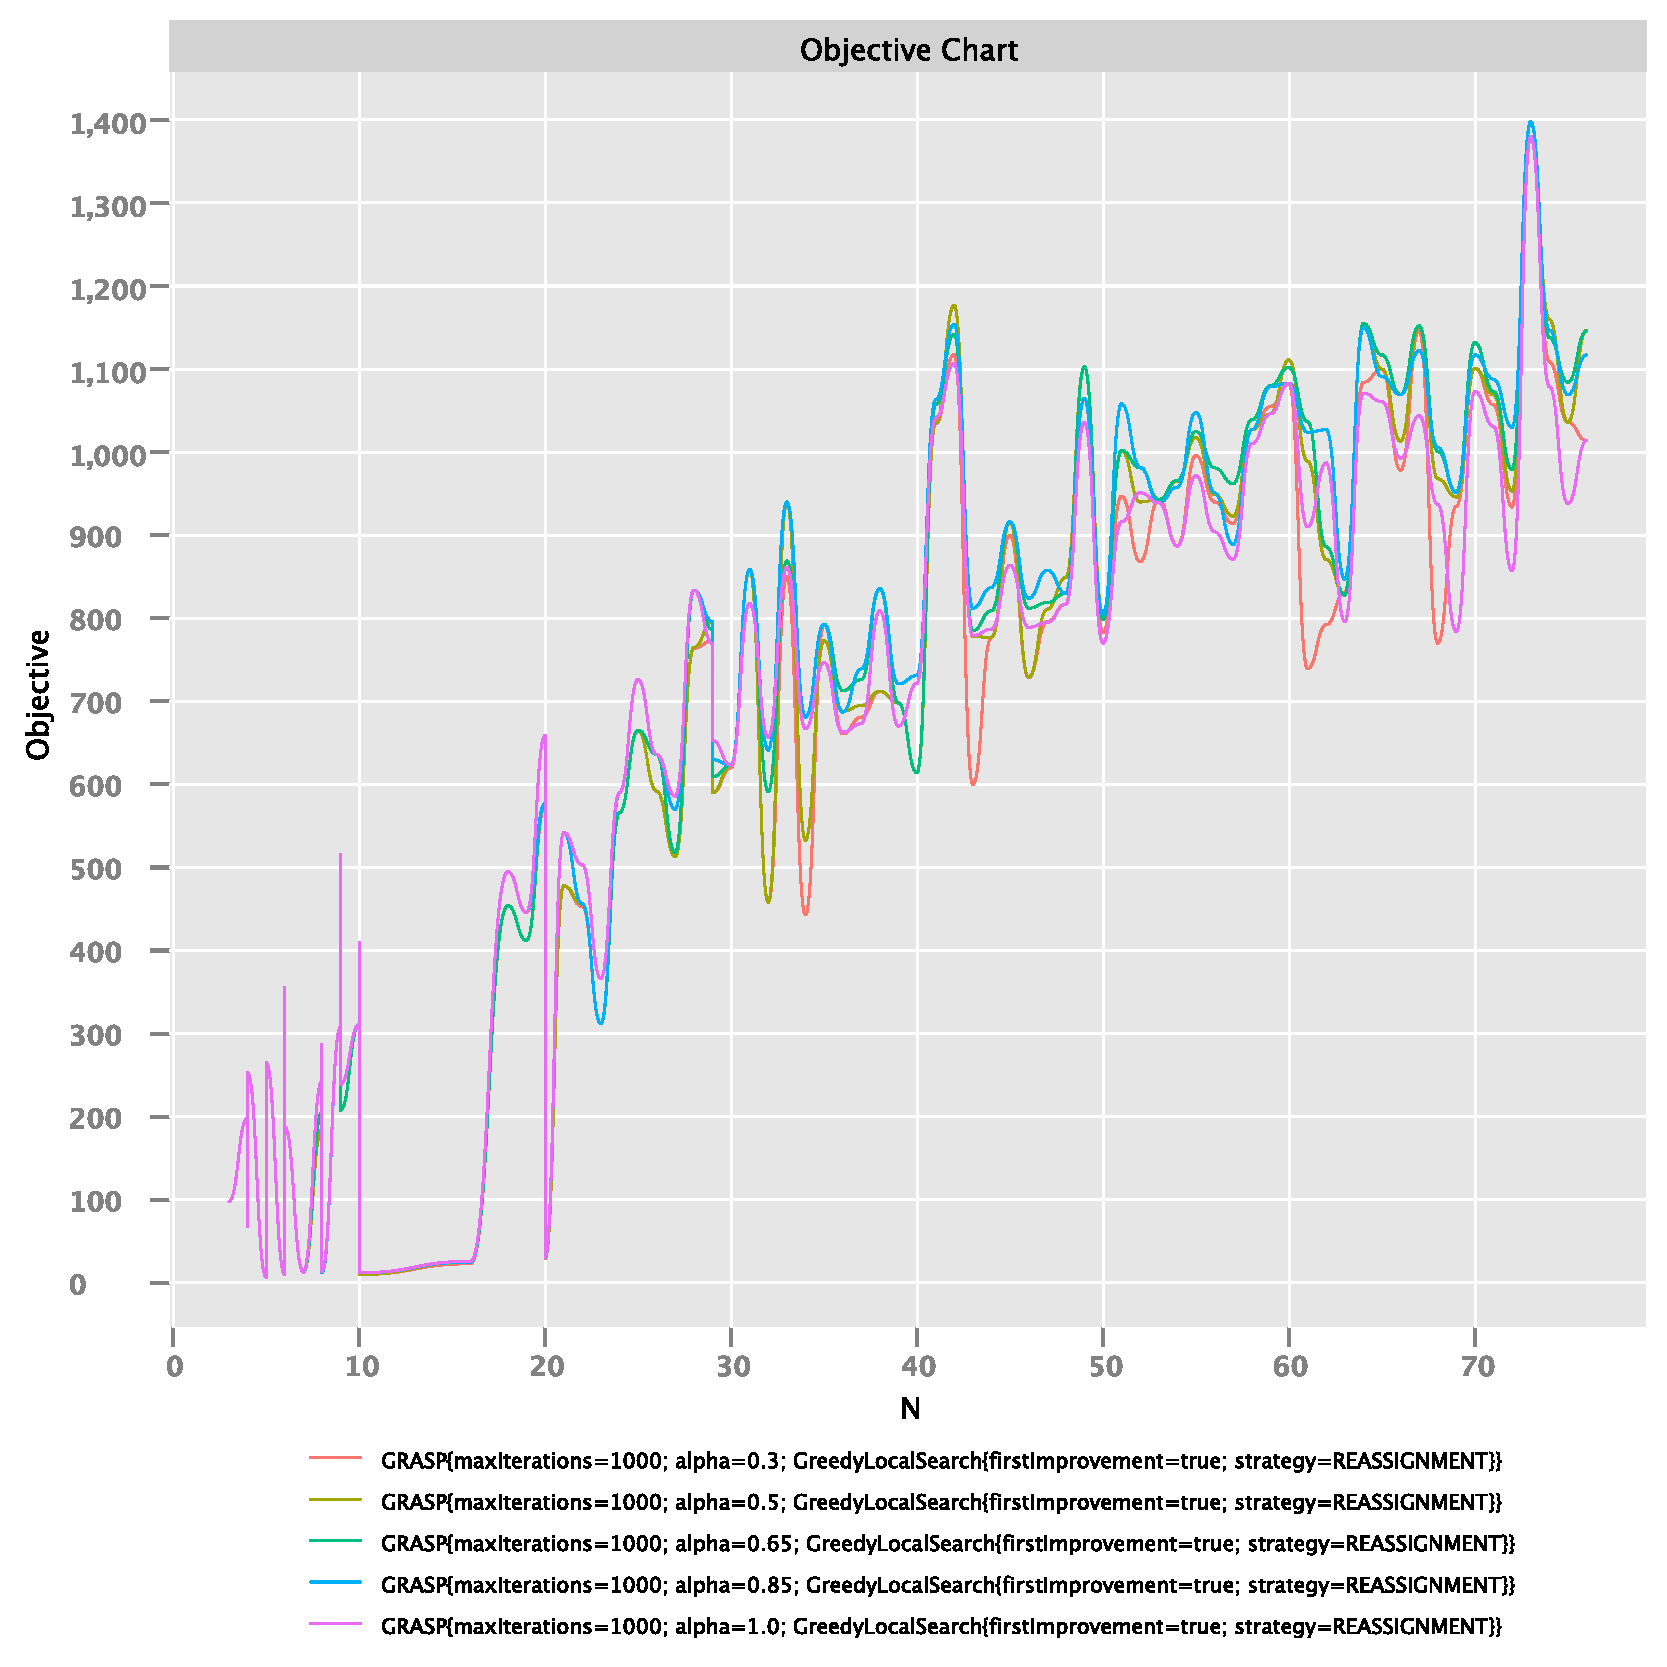
\includegraphics[width=0.8\textwidth]{./documentation/assets/new.GRASPParams.objectiveChart.pdf}
\end{frame}

\begin{frame}
\frametitle{All Time chart}
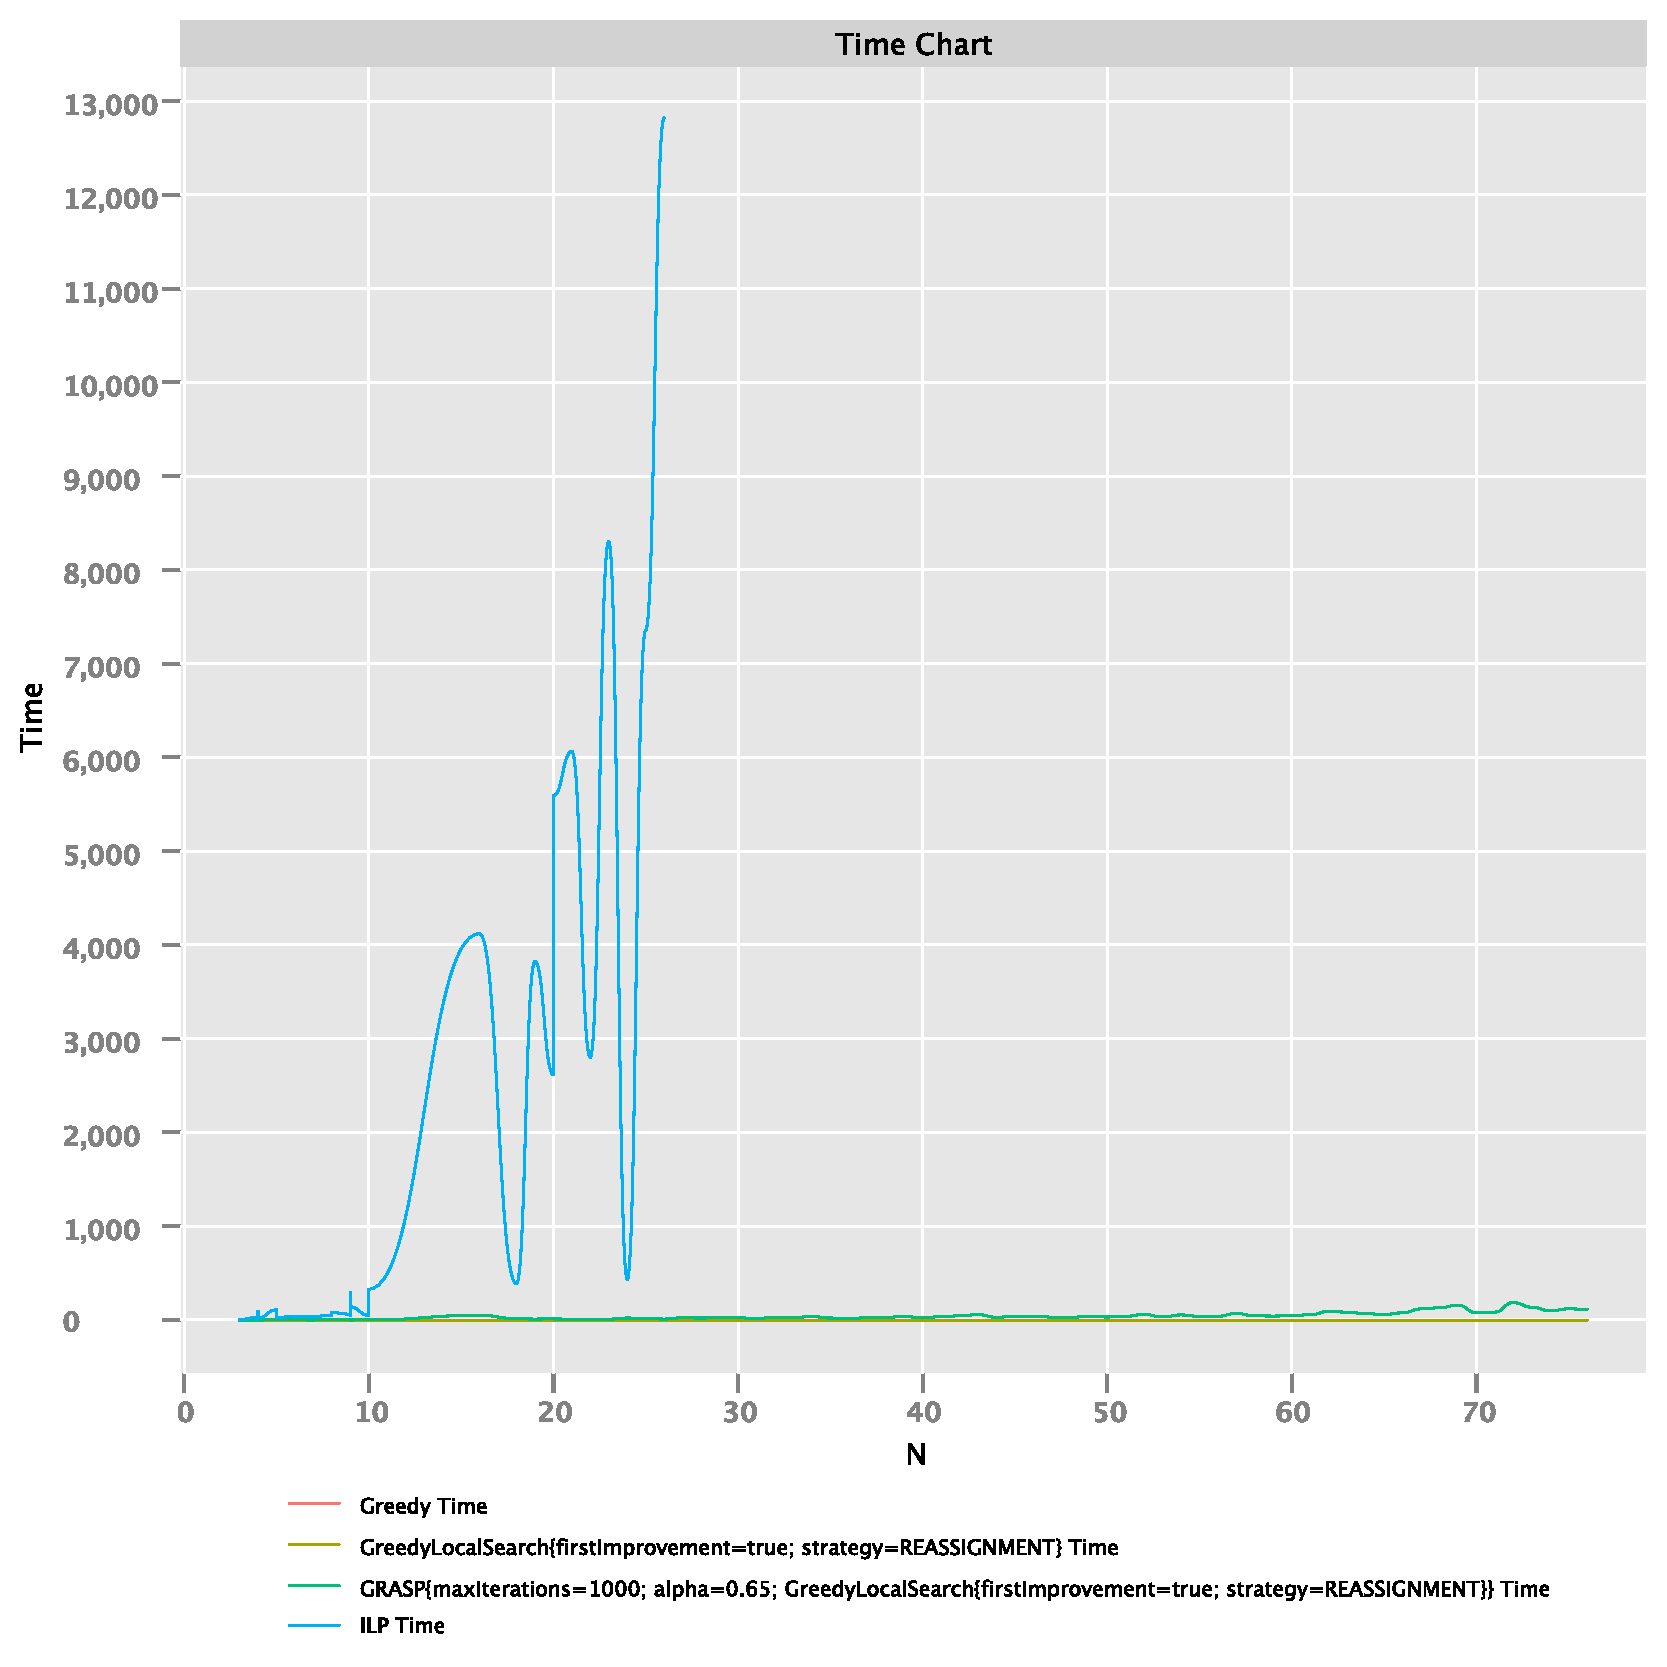
\includegraphics[width=0.8\textwidth]{./documentation/assets/new.all.timeChart.pdf}
\end{frame}

\begin{frame}
\frametitle{All Objective chart}
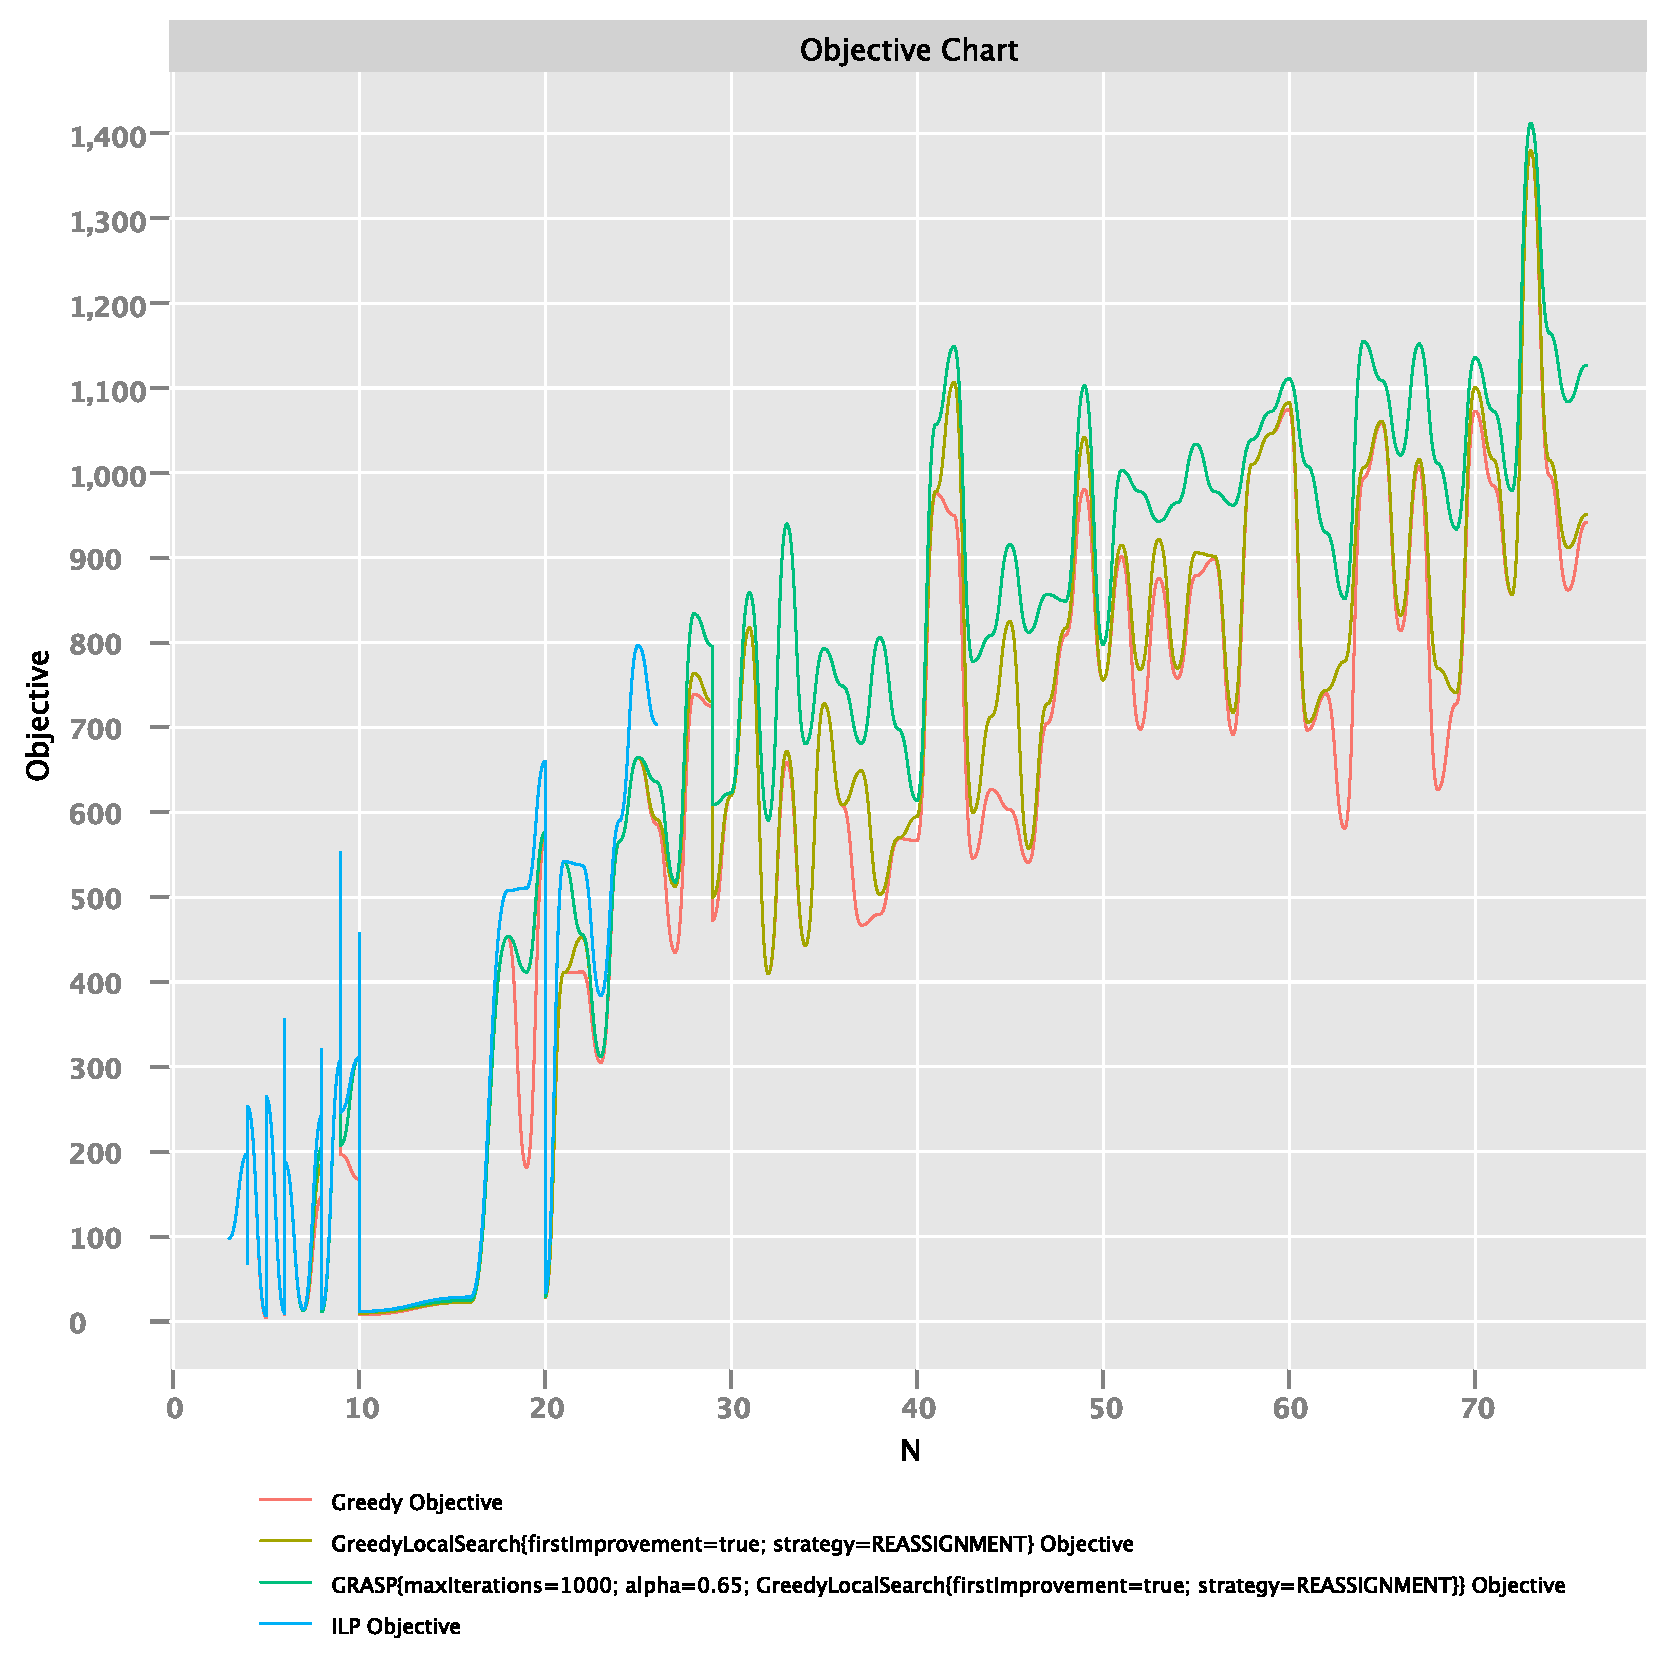
\includegraphics[width=0.8\textwidth]{./documentation/assets/new.all.objectiveChart.pdf}
\end{frame}

\begin{frame}
\frametitle{Improvements}
\begin{itemize}
    \item Parallelize algorithm
    \item Better strategies
    \item Implement the state of the art for heuristic
\end{itemize}
\end{frame}

\end{document}